\documentclass[11pt]{book}
\bibliographystyle{gerplain}
\setlength{\headheight}{10pt}
\usepackage[german, ngerman]{babel}
\usepackage{graphicx}
\usepackage{lscape}
\usepackage{caption}
\usepackage{longtable}
\usepackage{setspace}
\usepackage{listings}
\usepackage{ulem}
\usepackage{float}
\usepackage{titleref}


\usepackage{listings}

\lstset{language=JAVA, basicstyle=\small \ttfamily, showspaces=false, showtabs=false, tab= , keywordstyle=\bfseries, showstringspaces=false, framexleftmargin=5mm, frame=single, numbers=left, numberstyle=\tiny, stepnumber=1, numbersep=5pt, texcl=false, escapechar=$}
%-----------------------------------------------------------
% properties
%-----------------------------------------------------------
\author{Raffael Schmid} 


%-----------------------------------------------------------
% design
%-----------------------------------------------------------




%-----------------------------------------------------------
% document
%----------------------------------------------------------
\begin{document}
\begin{titlepage}
    \begin{center}
    \huge \textbf{\textsf{Erstellung eines Blueprints im Bereich Scala/Lift auf der Basis einer Applikation f\"ur die Ferienplanung}} \\
    \vspace{2cm}
    \LARGE\textbf{\textsc{Semesterarbeit}}\\
    \vspace{1cm}
    \normalsize
    vorgelegt am: xx. November 2010 \\
    \vspace{2.5cm}
    \large \textbf{an der Hochschule f\"ur Technik in Z\"urich}\\
    \vspace{5cm}
    \end{center}
 \normalsize{
    \begin{tabular}{ll}
    	Student: &Raffael Schmid, rschmid@hsz-t.ch\\
     	Dozent: & Beat Seeliger, seb@panter.ch \\
    	Studiengang: & Informatik\\
    \end{tabular}\\
    }
\end{titlepage}
\chapter*{Zusammenfassung}
Ziel dieser Semesterarbeit ist es, die M\"oglichkeiten und das Potential der Programmiersprache Scala respektive des Webframeworks Lift zu erforschen und das notwendige Knowhow zu erarbeiten. In erster Linie wurden Funktionalit\"aten wie die Persistenz, Internationalisierung und Support f\"ur RESTful Webservices untersucht. Daneben ging es aber auch um die Analyse von nichtfunktionalen Eigenschaften wie Architektur, Erweiterbarkeit, Deployment und Testbarkeit.

Zum Erreichen dieses Ziels wird auf der Basis von Lift und Scala eine Webapplikation zur Ferienplanung erstellt. Diese war urspr\"unglich als Basis f\"ur eine Software zur Ressourcenplanung gedacht - dient aber in erster Linie vorerst als ''Spielwiese'' um verschiedene Anforderungen der Zielsoftware zu diskutieren.

Die resultierende Webapplikation wurde mittels dem Webframework Lift als Backend implementiert, das Frontend besteht teils aus normalen HTML Seiten, teils aus in Flex \footnote{Flex ist ein Framework von Adobe mittels welchem man mit relativ geringem Zeitaufwand Webclients erstellen kann. http://www.adobe.com/de/products/flex} implementierten Komponenten welche via REST Schnittstelle auf die Services im Hintergrund zugreiffen. Zur persistierung wurde die Java Persistence API verwendet, als Implementation war Hibernate am naheliegensten. Lift selbst und auch darauf basierende Applikationen sind in Scala umgesetzt. Die Applikation l\"auft Produktiv in der STAX\footnote{http://www.stax.net} Cloud.
\tableofcontents
\chapter*{Einleitung}
W\"ahrend vielen Stunden habe ich mich mit Scala, dem Lift Webframework, dem Design eines Prototypen zur Ferienplanung, der entsprechenden Implementation und der Dokumentation besch\"aftigt. F\"ur mich waren die Technologien relativ neu, ich kannte sie nur aus der Theorie und wie sehr oft in der Informatik, aller Anfang war schwer.  Die ersten Versuche waren zwar wegbereitend, aber m\"uhsam. Die Einarbeitung in die verschiedenen Persistenz Frameworks war sehr aufw\"andig und ich war unmittelbar davor, auf ein mir bekanntes Webframework zu wechseln. Ich h\"atte dann das Ziel verfehlt, mir am Ende ein Bild von Scala und Lift machen zu k\"onnen. Die Prozesse der Applikation waren mir zu diesem Zeitpunkt schon relativ klar, trotzdem ging es jetzt an die Definition dieser,  ans erstellen eines passenden Rollenkonzepts, Navigation und basierend auf diesen Vorgaben zu Design und anschliessend Implementation des Dom\"anenmodells mit JPA. Nun war es relativ schnell m\"oglich, Objekte in der Datenbank zu persistieren und dem lang ersehnten Flow stand nichts mehr im Wege. Der Planung lief ich zu diesem Zeitpunkt leider schon etwas hinterher, denn im Allgemeinen habe ich mir unter ``fast to build''\cite{liftweb} einen einfacheren Einstand vorgestellt. Trotzdem, gegen Ende schwanden die Wolken am Horizont, es entstand eine gewisse Hingabe und ich \"uberlege mir, wo ich Scala oder Lift als n\"achstes einsetzen k\"onnte. Hoffentlich hilft die eine oder andere Feststellung auch weiteren Leuten oder ich kann jemanden f\"ur Scala oder Lift begeistern.

Das Dokument der Semesterarbeit ist in drei Teile gegliedert. Teil eins mit der Aufgabenstellung, Teil zwei mit deren Analyse, den zur Implementation ben\"otigten Grundlagen, Design und Konzeption, Implementation sowie der Beschreibung von Entwicklungs- und Testumgebung. Anschliessend folgt im dritten Teil der R\"uckblick, hier wird die Applikation anhand der Vorgaben bewertet und ein Fazit \"uber die verwendeten Technologien gezogen. \newline\newline
Danke f\"urs Interesse\newline
Raffael Schmid

\part{Projektdetails}
\chapter{Aufgabenstellung}
\section{Ausgangslage}
In vielen Firmen, welche ohne ERP Software auskommen, wird die Planung von Ressourcen manuell mit der Hilfe verschiedenster Standardsoftware (Excel, Access) oder Papier gemacht. Was in vielen Projekten, Unternehmen fehlt, ist die Software zur Planung von Ressourcen. Als Grundlage dazu soll ein webbasierter Ferienplaner implementiert werden, der sp\"ater sukzessive zu einer Gesamtl\"osung erweiter werden kann. Zur Implementierung dieses Prototypen wird das Lift Webframework verwendet. Lift \footnote{http://liftweb.net} ist ein Framework auf der Basis von Scala (eine Programmiersprache die mitunter an der Ecole Polytechnique Fédérale de Lausanne entwickelt wurde) und verinnerlicht auch deshalb in vielen Bereichen v\"ollig neue Konzepte. Der Prototyp soll auch die M\"oglichkeiten der doch eher neueren Bibliothek transparent darstellen. Ich m\"ochte darauf hinweisen, dass ich mir zus\"atzlich zum Prototypen das Knowhow im Bereich Scala und Lift erarbeiten muss. Die Arbeit soll es mir erm\"oglichen, eine Aussage \"uber das Potential von Lift machen zu k\"onnen. Scala hat, wenn man sich auf Magazine oder verschiedenster Internetseiten wie zum Beispiel den Tiobe-Index \footnote{http://www.tiobe.com/index.php/content/paperinfo/tpci/index.html} bezieht, den Durchbruch ja schon fast geschafft. 

\section{Ziel der Arbeit}
Als Vorarbeit zur Konzeption und Entwicklung dieses Prototypen muss das Knowhow im Bereich Lift respektive Scala erarbeitet werden. Bei diesem Prozess stehe ich zwar nicht mehr am Anfang, ich werde jedoch trotzdem zus\"atzlich Zeit zum Aufbau meines Wissens ben\"otigen. Darauf aufbauend werden die Requirements der Applikation definiert und entsprechende Konzepte erstellt (User, Rollen, Prozesse). Aufgrund dieser Requirements werden Recherchen durchgef\"uhrt, um herauszufinden, ob Konzepte oder Teile bestehender L\"osungen \"ubernommen werden k\"onnen. Anschliessend werden die Requirements des Prototypen umgesetzt. 

\subsection{Optionale Ziele}
Ich erwarte, dass diese Zielsetzung den Rahmen einer Semesterarbeit bereits deckt, f\"ur den Fall dass ich noch Zeit finde, fasse ich optional noch folgende Punkte ins Auge: 

\begin{enumerate}
	\item Setup von Test- und Produktiver Umgebung
	\item Performance Testing
	\item Internationalization 
	\item Search Engine Optimization
	\item Usability
\end{enumerate}

\section{Aufgabenstellung}
Erarbeitung einer Wissensbasis im Bereich Lift und Scala, um die Konzeption und Implementation des Prototypen zu erm\"oglichen. Setup der Entwicklungs-Infrastruktur. Dies beinhaltet das Projektsetup mit Maven, Versionskontrolle mit Git oder Subversion, Einrichten der Entwicklungsumgebung, Aufsetzen Infrastrukur f\"ur automatisierte Testl\"aufe, Entwicklungsserver, allerdings werde ich auf den Einsatz einer Continuous Integration Software verzichten. W\"ahrend der Konzeption werden Navigations- und Rollenkonzepte erstellt sowie die verschiedenen Prozesse definiert. Implementation des Prototypen beinhaltet unter anderem Folgendes:

Aufbau des Domain Modells - Implementation der Persistenz-Schicht - Security: Registrierung, Login, ... - Navigation - Mail-Versand - Evaluierung eines geeigneten, auf Javascript basierendem Kalender, um die Pers\"onliche Ferien\"ubersicht sowie die Team\"ubersicht darstellen zu k\"onnen.

\section{Erwartetes Resultat}
Dokumentation der Semesterarbeit beinhaltet unter anderem folgende Teile: 
\begin{itemize}
\item Konzepte
	\begin{itemize}
		\item Navigationskonzept
		\item Rollenkonzept
		\item Prozesse Dokumentation
	\end{itemize}	
	\item Implementationsdetails
	\item Entscheide Software
	\item Lauff\"ahige Software als Maven-Projekt
\end{itemize}





\part{Umsetzung}
\chapter{Analyse der Aufgabenstellung}
\section{Idee und Ziele der Arbeit}
Das grunds\"atzliche Ziel hinter der vorgelegten Semesterarbeit war es, sich mit dem Lift Webframework und Scala auseinander zu setzen um im Anschluss daran eine Aussage dar\"uber machen zu können, ob sich die beiden Technologien in naher Zukunft als Plattform zur Entwicklung einer Webseite anbieten w\"urden. Zu Beginn steht auch die Erarbeitung des Knowhows in den beiden Bereichen Scala (siehe Abschnitt \ref{einarbeitung:scala} \titleref{einarbeitung:scala}) , Lift (siehe Abschnitt ''\ref{einarbeitung:lift} \titleref{einarbeitung:lift}'' im Zentrum. In der Folge sind die aus der Aufgabenstellung entstehenden Ziele definiert.

\subsection{Vorbereitung: Erarbeitung des Basiswissens}
Nebst dem Projekt-Setup und der Einarbeitung in Scala (siehe dazu Abschnitt \ref{einarbeitung:scala} \titleref{einarbeitung:scala})  besteht ein wesentlicher Bestandteil dieses Punktes auch darin, herauszufinden wie die folgenden Problemstellungen, die sich bei der Idee des Ferienplaners nicht wesentlich von anderen Punkten unterscheiden, mit Lift umsetzen lassen:
	\begin{itemize}
		\item Authentifizierung, Authorisierung
		\item Persistenz respektive Objekt-Relationales Mapping
		\item Internationalisierung
	\end{itemize}
Die soeben beschriebenen Punkte sind im Abschnit \ref{einarbeitung:lift} \titleref{einarbeitung:lift} dokumentiert.

\subsection{Design}
Nachdem die Einarbeitung abgeschlossen ist, kann mit dem Design der Arbeit begonnen werden. Dieser Punkt beinhaltet zum einen die Definition der Prozesse und zum anderen das Design des Datenbank Schemas. Beide Punkte sind angesichts der \"uberschaulichen Problemstellung des Ferienplaners zeitlich nicht sehr aufw\"andig.

\subsection{Technische Umsetzung}
Im Anschluss an die Design-Phase wird der Prototyp umgesetzt. Die Details zur Umsetzung befinden sich im Abschnitt \ref{implementation} \titleref{implementation}.


\section{Lieferumfang der Semesterarbeit}
\subsection{Dokumentation}

Ausgehend von der Aufgabenstellung muss die Dokumentation folgende Teile beinhalten:
\begin{itemize}
	\item Konzepte
	\begin{itemize}
		\item Navigationskonzept befindet sich im Abschnitt \ref{konzept:navigation} \titleref{konzept:navigation}.
		\item Rollenkonzept befindet sich im Abschnitt \ref{konzept:rollen} \titleref{konzept:rollen}.
		\item Die Definitionen der Prozesse befinden sich Abschnitt \ref{konzept:prozesse} \titleref{konzept:prozesse}
	\end{itemize}
	\item Implementationsdetails befinden sich im Abschnitt \ref{implementation} \titleref{implementation}
\end{itemize}
(aufgeteilt in Navigationskonzept, Rollenkonzept und Prozesse) und die Details zur Implementation (inklusive Begr\"undung, weshalb wann welche Technologien oder Module verwendet wurden) beinhalten. 

\subsection{Prototyp}
Die Definition des Wortes Prototyp ist bekanntlich ein bisschen schwammig. In meinem Sinne sollte der Prototyp die folgenden Punkte erf\"ullen:

\begin{enumerate}
\item \textbf{Potential} - Anhand der Implementation des Prototypen solle eine qualifizierte Aussage dar\"uber gemacht werden, wie viel Potential in Scala und Lift steckt. 

\item \textbf{Erkenntnisse} - In den tangierten Bereichen (Persistenz, Webservices, usw.) sollen Ans\"atze von Best Practices erarbeitet werden k\"onnen respektive Aussagen \"uber die Vor- und Nachteile von verschiedenen Technologien gemacht werden k\"onnen. Dies betrifft auch die Bereiche Entwicklungsumgebung, Build-Tools, usw.

\item \textbf{Abdeckung des Funktionsumfangs} - Ich werde versuchen, einen m\"oglichst grossen Funktionsumfang der Applikation zu implementieren.
\end{enumerate}







\chapter{Grundlagen}
\section{Funktionale Programmierung}
Um das Prinzip der Funktionalen Programmierung ein kurzer Vergleich zwischen imperativer und deklarativer Programmierung.
\subsection{Imperativ vs. Deklarativ}
Im Gegensatz zu den Imperativen\footnote{der Begriff Imperativ bezeichnet die Befehlsform (lat: imperare=Befehlen)} Sprachen wird der ''Computer'' angewiesen, wie er ein bestimmtes Resultat berechnen muss. Die Deklarativen Sprachen hingegen erm\"oglichen eine Trennung zwischen Arbeits- und Steuerungsalgorithmus. Wir formulieren, was wir haben wollen, und m\"ussen dazu nicht wissen, wie es im Hintergrund ''erarbeitet'' wird.

Als gutes Beispiel f\"ur eine deklarative Sprache ist SQL, die Structured Query Language zur Abfrage von Daten einer Datenbank, und ist deshalb ein gutes Beispiel f\"ur eine Sprache die unserem Denken entspricht. 

\begin{lstlisting}[caption=Sql Deklaration]
select first_name, last_name, zip, city 
from tbl_user 
where zip<=8000;
\end{lstlisting}


  \begin{longtable}{|p{2cm}|p{2cm}|p{2cm}|p{2cm}|}
    \caption{Resultat der deklarativen Abfrage}\\
\hline
  firstname & lastname & zip & city\\
  \hline
    Flavor & Flav & 8000 & Z\"urich\\
  \hline
  \end{longtable}

Eine Sql-Anweisung ist im Normalfall auch ohne detaillierte Erkl\"arung verst\"andlich und man hat sich nicht mit dem Steuerungsalgorithmus im Hintergrund zu besch\"aftigen. Da die Queries nur auf Tabellen operieren, m\"ussen wir nicht einmal wissen, wie Computer funktionieren. Mit Hilfe der Abfragesprache k\"onnen wir uns auf das Wesentliche konzentrieren und mit wenigen Anweisungen viel erreichen. \cite{Piepmeyer201006}

Im Gegensatz zu dieser Deklaration ist beispielsweise die Aufsummierung aller Zahlen einer Liste in Sprachen wie Java, C++ oder C\# imperativ:

\begin{lstlisting}[caption=Summe einer Liste in Java]
List<Integer> summanden = asList(new Integer[] { 1, 2 });
int summe = 0;
for (int i = 0; i < summanden.size(); i++) {
	summe = summe + summanden.get(i);
}
System.out.println(summe);
\end{lstlisting}

Imperative Sprachen haben unter anderem die folgenden Eigenschaften:
\begin{itemize}
\item Programme bestehen aus Anweisungen, die der Prozessor in einer bestimmten Reihenfolge abarbeitet. If-Else-Anweisungen werden durch Forw\"artsspr\"unge realisiert, Schleifen durch R\"uckw\"artsspr\"unge.
\item Werte von Variablen ver\"andern sich unter umst\"anden kontinuierlich.
\end{itemize}

In h\"oheren Sprachen wie zum Beispiel Scala wird die Berechnung der Summe auf deklarative Weise gemacht und sieht folgendermassen aus:
\begin{lstlisting}[caption=Summe einer Liste in Scala]
List(1,2,3).foldLeft(0)((sum,x) => sum+x)
\end{lstlisting} 

\subsection{Funktionale Programmierung}
Funktionale Programmierung besitzt die folgenden eigenschaften:
\begin{itemize}
\item jedes Programm ist auch eine Funktion
\item jede Funktion kann weitere Funktionen aufrufen
\item Funktionale Sprachen haben Top-Class Funktionen welche nicht nur definiert und aufgerufen werden k\"onnen, sondern als Werte respektive Objekte herumgereicht werden k\"onnen.
\item Die theoretische Grundlage von Funktionaler Programmiersprachen basiert auf dem Lambda-Kalk\"ul\footnote{Der Lambda-Kalk�l ist eine formale Sprache zur Untersuchung von Funktionen. Sie beschreibt Funktionsdefinitionen, das Definieren formaler Parameter sowie das Auswerten und Einsetzen aktueller Parameter. http://de.wikipedia.org/wiki/Lambda-Kalk\"ul} Jeder Ausdruck wird dabei als auswertbare Funktion betrachtet, so dass Funktionen als Parameter �bergeben werden k�nnen.
\end{itemize}





\section{Statisch typisierte Sprachen}
Statisch typisierte Sprachen zeichnen sich dadurch aus, dass sie im Gegensatz zu dynamisch typisierten Sprachen den Typ von Variablen schon beim Kompilierungsprozess ermitteln. Dies kann im wesentlichen durch 2 verschiedene Arten geschehen:

\subsection{Explizite Deklaration und Typinferenz}
Bei der expliziten Deklaration wird der Typ einer Variablen respektive der R\"uckgabetyp einer Funktion festgelegt und wird f\"ur die weitere Verwendung bekannt gemacht. Im Normalfall k\"onnen diese expliziten Definitionen aus den restlichen Angaben hergeleitet werden und k\"onnen in h\"oheren Sprachen wie beispielsweise Scala weggelassen werden - dann Spricht man von Typinferenz. Die heutigen Programmiersprachen besitzen unterschiedliche F\"ahigkeiten in Sachen Typinferent. 

\subsubsection{Typinferenz in der Praxis}
In Sachen Typinferenz ist Java wenige beg\"utert. Ein kleines Beispiel welches das kleine bisschen Typinferenz in Java aufzeigen soll:

\begin{lstlisting}[caption=Typeinferenz in Java]
public static void main(String[] args) {
	List<String> list = newArrayList();
}
public static <T> List<T> newArrayList() {
	return new ArrayList<T>();
}
\end{lstlisting}
Die Ermittlung des R\"uckgabetyps aufgrund des Variablen-Typs ist schon fast alles was Java in Sachen Typeinferenz zu bieten hat. Etwas mehr kann mit den h\"oheren Sprachen wie Scala erreicht werden:
\begin{lstlisting}[caption=Typeinferenz in Scala]
scala> val s = "inference"
s: java.lang.String = inference

scala> val l = List("a","b","c")
l: List[java.lang.String] = List(a, b, c)
\end{lstlisting}

\subsection{Vorteile von statischer Typisierung}
\begin{itemize}
\item Bestimmte Fehler werden durch die Typpr\"ufung w\"ahrend der Kompilierzeit vermieden.
\item Grunds\"atzlich ist das akribische Testen von Code weniger wichtig. 
\item Die Performance von statisch typisierten Sprachen ist deshalb besser, weil die ermittlung des Typs zur Laufzeit in den meisten F\"allen vermieden werden kann.
\end{itemize}

\subsection{Nachteile von statischer Typisierung}
\begin{itemize}
\item Dynamische Sprachen erm\"oglichen eine h\"ohere Flexibilit\"at. Zum Beispiel k\"onnen folgende Dinge in statischen Sprachen nicht, mit erh\"ohtem Aufwand oder mit schlechtem Design gemacht werden:
\begin{itemize}
\item Einf\"ugen von Methoden in Classen oder Objekte zur Laufzeit.
\item Duck Typing\footnote{Duck-Typing ist ein Konzept der objektorientierten Programmierung, bei dem der Typ eines Objektes nicht durch seine Klasse beschrieben wird, sondern durch das Vorhandensein bestimmter Methoden. http://de.wikipedia.org/wiki/Duck-Typing}
\end{itemize}
\item Kompilieraufwand ist wesentlich gr\"osser.
\end{itemize}
\subsection{Scala und die Typisierung}






\chapter{Design und Konzeption}
Nach der Analyse der Aufgabenstellung und der Erarbeitung des Knowhows im Bereich von Scala und des Lift Frameworks ging es an Design und Konzeption. In dieser Phase entstanden auf der Basis von \ref{konzept:usecase} \titleref{konzept:usecase} die in der Aufgabenstellung definierten Konzepte der Benutzerrollen, Navigationskonzept und der Prozesse. Als Basis f\"ur die Implementation dient zum Ende \ref{design:erm} \titleref{design:erm} und \ref{design:architektur} \titleref{design:architektur}
\section{Use Cases Beschreibung}\label{konzept:usecase}
 \begin{figure}[H]
  	\centering
    	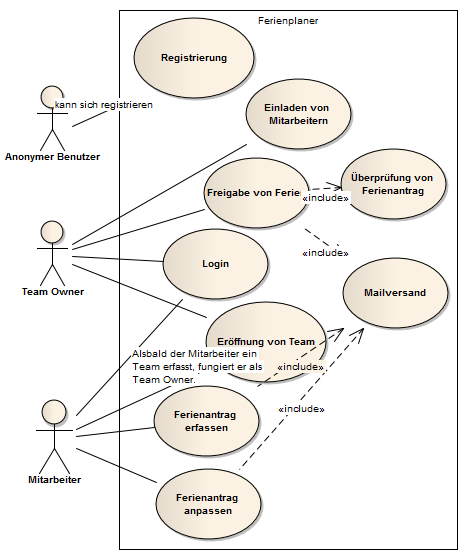
\includegraphics[width=13cm]{images/usecases}
 	\caption{Use Case Diagramm}
\end{figure}
\subsection{Aktoren}
\subsubsection{Mitarbeiter} sind registrierte Benutzer und k\"onnen von Team Ownern zu den entsprechenden Teams hinzugef\"ugt werden. 
\subsubsection{Owner - Team Owner} sind grunds\"atzlich auch Mitarbeiter, die allerdings ein eigenes Team administrieren und f\"ur dieses (es k\"onnen auch mehrere sein) deshalb zus\"atzliche Kompetenzen besitzen.

\subsection{Beschreibung der Use Cases}
\subsubsection{Projekt er\"offnen}
Nach dem Login erfasst der Administrator (Project Manager, Teamleiter, usw.) f\"ur sein Team ein Projekt. Grunds\"atzlich geh\"ort ein Projekt mehreren Administratoren, in einem 2. Projekt wird die zus\"atzliche M\"oglichkeit implementiert, anderen Benutzer Administrator-Rechte f\"urs eigene Projekt zu geben.

\subsubsection{Mitarbeiter in Projekt erfassen}
Projekte alleine sind leere ''Beh\"alter'' f\"ur Mitarbeiter. Um Mitarbeiter ins eigene Projekt zu nehmen, sucht der Administrator nach einem bestehenden User. Sofern es den gesuchten Benutzer im System noch nicht gibt, wird er durch den Administrator neu erfasst. Der neu erfasste Benutzer wird mittels Mail auf diese Aktion aufmerksam gemacht.

\subsubsection{Ferienw\"unsche bearbeiten}
Die vom Mitarbeiter erfassten Ferien k\"onnen durch den Administrator bez\"uglich Status und Termin ver\"andert werden. Die Bewilligung von Ferien wird mittels des Status confirmed / best\"atigt erteilt. Ansonsten gibt es folgende M\"oglichkeiten:
\begin{itemize}
\item erw\"unscht - requested
\item abgelehnt - rejected
\item best\"atigt - confirmed
\end{itemize}

\subsubsection{Ferienwunsch erfassen}
Der Mitarbeiter kann seine Ferienw\"unsche pro Projekt erfassen. Diese befinden sich zu Beginn im Status ''requested'' und k\"onnen vom Administrator in die Status ''rejected'' und ''confirmed'' ge\"andert werden.

\subsubsection{Ferienwunsch bearbeiten}
Sollte ein Ferienwunsch abgelehnt werden, kann er erneut bearbeitet werden, was eine erneute Anfrage beim Administrator zur Folge hat.

\section{Rollen-Konzept}\label{konzept:rollen}
Im Grunde handelt es sich bei dem Ferienplaner um einen Prototypen ohne eigentlichen Business Case im Hintergrund. Aus diesem Grund sehe ich als Anfang nur 2 Rollen vor. Zum einen ist es der Anonyme Benutzer, der zwar die Webseite Besuchen kann, sich f\"ur die weiteren Schritte allerdings registrieren muss, zum anderen ist es der Registrierte Benutzer, der nicht nur Ferien erfassen, sondern auch eigene Teams mit eigenen Mitarbeitern bilden kann. Als Business Case k\"onnte ich mir vorstellen, dass es eine Trennung des Owners vom Mitarbeiter gibt, und daf\"ur spezielle Bedingungen (z.B. Bezahlung, etc.) erf\"ullt werden m\"ussen.
\subsection{Anonymous}
Folgende Funktionalit\"aten stehen dem Anonymous zur Verf\"ugung:
\begin{itemize}
\item Ansicht von \"offentlichen Seiten
\item Registrierung
\end{itemize}

\subsection{Registrierte Benutzer}
Nebst den Funktionen des Anonymous stehen dem Registrierten Benutzer folgende Dinge zur Auswahl:
\begin{itemize}
\item Login
\item Administration von Teams und Zuweisung von Mitarbeitern
\item Einladen von Mitarbeitern
\item Erfassen von Ferien f\"ur Teams welchen der Registrierte Benutzer angeh\"ort.
\end{itemize}

\subsection{Optional Aufteilung der Registrierten Benutzer}
Bei allf\"alligem Business Case best\"unde die M\"oglichkeit, die Rolle des Registrierten Benutzers in Mitarbeiter und Team Owner aufzuteilen. In diesem Falle h\"atte man die M\"oglichkeit, bestimmte Richtlinien (Zahlungsrichtlinien, etc.) zu errichten. Als Beispiel w\"urden die Rollen folgendermassen aussehen:
\subsubsection{Mitarbeiter}
Folgende Funktionalit\"aten stehen dem Mitarbeiter zur Verf\"ugung:
\begin{itemize}
\item Erfassen von Ferien f\"ur Teams welchen der Registrierte Benutzer angeh\"ort.
\end{itemize}

\subsubsection{Team Owner}
Zus\"atzlich zu den Funktionen des Mitarbeiters kann der Team Owner folgendes tun:
\begin{itemize}
\item Administration von Teams und Zuweisung von Mitarbeitern
\item Einladen von Mitarbeitern
\end{itemize}

\section{Prozesse}\label{konzept:prozesse}
\subsection{Person registrieren}
 \begin{figure}[H]
  	\centering
    	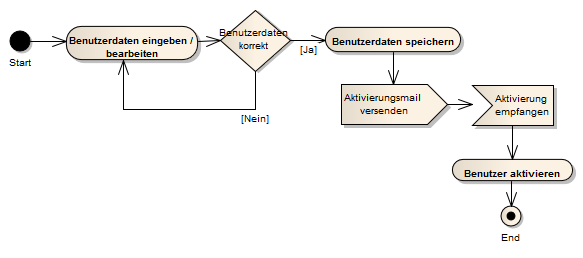
\includegraphics[width=15cm]{images/process_registration}
 	\caption{Prozess Member Administration Webpage}
\end{figure}

\subsection{Ferien beantragen, planen}\label{prozess:ferien}
 \begin{figure}[H]
  	\centering
    	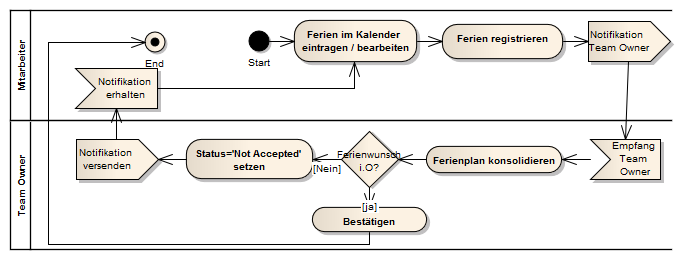
\includegraphics[width=15cm]{images/process_vacation}
 	\caption{Prozess Ferien beantragen, planen}
\end{figure}


\subsection{Team administrieren}\label{prozess:team}
 \begin{figure}[H]
  	\centering
    	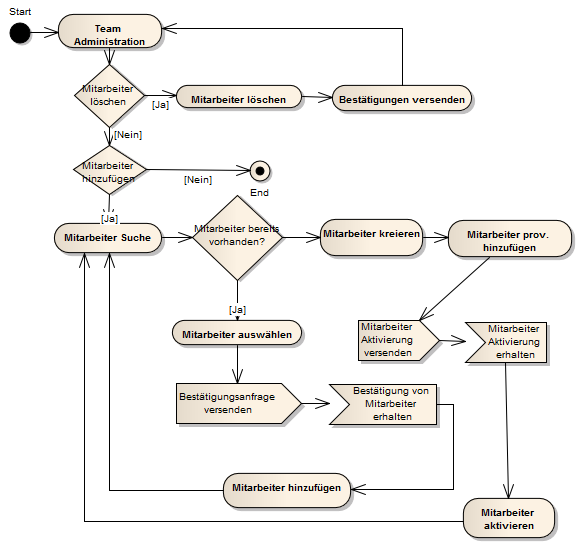
\includegraphics[width=15cm]{images/process_team_administration}
 	\caption{Prozess Member Administration Webpage}
\end{figure}

\section{Navigations-Konzept}\label{konzept:navigation}
 \begin{figure}[H]
  	\centering
    	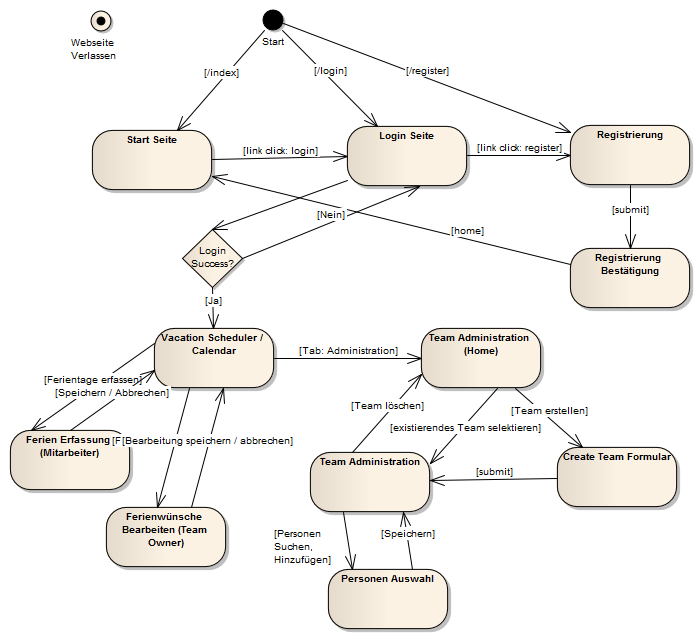
\includegraphics[width=13cm]{images/navigation_process}
 	\caption{Navigation Webpage}
\end{figure}

\section{Datenbank-Schema}\label{design:erm}

\subsection{Entity Relationship Model}
\begin{landscape}
 \begin{figure}
  	\centering
    	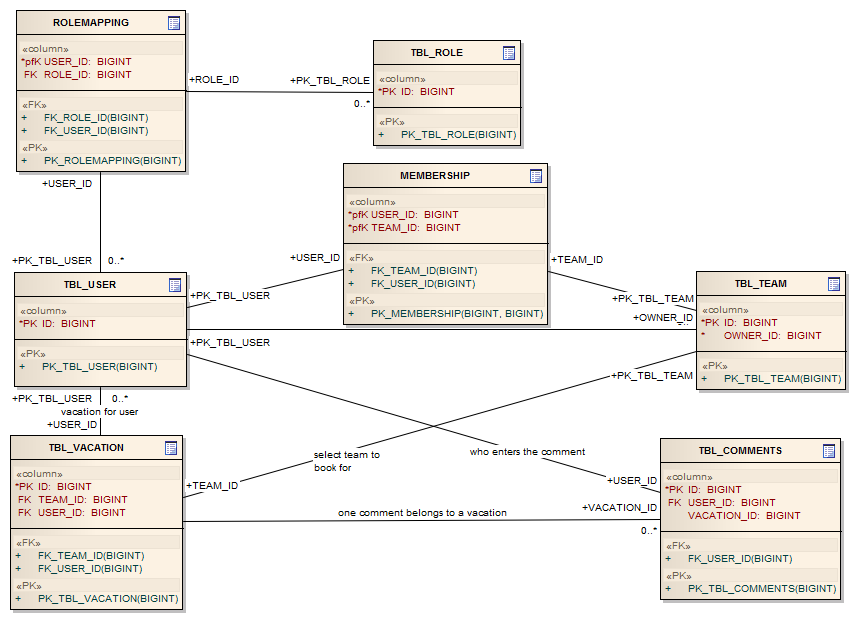
\includegraphics[width=19cm]{images/erm}
        	\caption{Entity Relationship Model}
\end{figure}
\end{landscape}
\subsection{Beschreibung}
Das Entity Relationship Model zeigt alle Tabellen, wie sieauf Ebene der Datenbank geplant sind. Many-to-Many Beziehungen sind also bereits aufgel\"ost. 

\subsubsection{User und Rollen}
Beginnen wir mit den Tabellen User und Rollen: F\"ur die Modellierung der Rollen gibt es meines Erachtens zwei vertretbare Alternativen. Erstens wie hier im ERM aufgezeigt, werden die Rollen via eine Join Table dem User zugewiesen. Die Erweiterung davon w\"are dann eine Zus\"atzlichen Self-Join auf der Tabelle TBL\_ROLE, damit man eine Hierarchie der Rollen abbilden kann, und Rollen den Benutzern auch in Gruppen zuweisen kann. Aufgrund der zus\"atzlichen Komplexit\"atsstufe habe ich mich f\"ur Variante eins entschieden.

\subsubsection{Teammitgliedschaft, Membership}
Die Zuteilung von Membern zu Teams muss ebenfalls \"uber eine Many-to-Many Assoziation realisiert werden. Im Diagramm ersichtlich an der Tabelle MEMBERSHIP. 

\subsubsection{Teamzugeh\"origkeit}
Im von mir modelierten einfacheren Fall, bei dem ein Team nur einem Verantwortlichen zugeteilt wird, wird die Beziehung zwischen TBL\_TEAM und TBL\_USER mittels einer One-To-Many Relation hergestellt. Nebst der Einfachheit hat dies den Nachteil, dass Ferien nur vom Ersteller und Team-Owner bewilligt werden k\"onnen, er kann also keine Stellvertreter daf\"ur nominieren. 

\subsubsection{Ferien}
Ferien werden als Eintr\"age in der Tabelle TBL\_VACATION definiert. Die Beziehung zu TBL\_USER ist relativ einleuchten, da diese immer einem Teilnehmer zugeordnet werden. Die Relation zu TBL\_TEAM kommt daher, weil ich Ferien immer \"fur ein spezifisches Team erfassen muss. Ob das dann manuell durch den Benutzer oder Applikatorisch f\"ur alle Teams durchgef\"uhrt wird, sei dahin gestellt. Jedenfalls, sofern ein Benutzer mehreren Teams zugeordnet ist, m\"ussen f\"ur all diese Teams Ferien-Records vorhanden sein.
\chapter{Implementation des Prototypen}\label{implementation}

\section{Architektur, Technologiewahl}
\subsection{Dependency Injection}\label{implementation:di}

\begin{lstlisting}[caption=Abh\"angigkeiten abh\"angig von der Umgebung]
object Beans {
  lazy val env = System.getProperty("run.mode")
  def init = {
    env match {
      case "test" =>
        Context.put[SecurityService]{()=>
            MockSecurityService}
      case _ =>
        Context.put[SecurityService]{()=>
            SecurityServiceImpl}
     }
  }
}
\end{lstlisting}
Das Dependency Management wurde mittels der im Abschnitt ``\ref{lift:di} \titleref{lift:di}'' Verfahren implementiert. Mittels der oben beschriebenen Bean-Definition die sich im Objekt bootstrap.config.Beans befindet ist es m\"oglich, je nach definiertem Environment (test, prod) eine die Objekte innerhalb des Bean-Contextes unterschiedlich zu definieren. Die oben beschriebenen Closures werden jedes mal aufgerufen, wenn eine Variable aus dem Context injected werden soll. Da hier ein Scala Objekt zur\"uckgeliefert wird, ist die Instanz vom Typ SecurityService zur Laufzeit nur einmal vorhanden. Bei Spring oder \"ahnlichen Frameworks spricht man vom ``Singleton Scope''. Liefert man ein neues Objekt zur\"uck, entspricht das Verhalten dem ``Prototype Scope bei Spring''. Der Lift-Injection bietet auch die M\"oglichkeit, Request- und Session-Scoped Objekte zu speichern. Als Beispiel, wie eine Variable vom Context angefordert wird die folgende Deklaration:

\begin{lstlisting}[caption=Anfrage einer Variable aus dem Lift Bean Context]
val securityService = Context.inject_![SecurityService]
\end{lstlisting}


\subsection{Persistenz}
\subsubsection{Evaluation des Persistenz Frameworks}
Bereits zu Beginn stellte sich die Frage, warum man welche der drei m\"oglichen und im Abschnitt ``\ref{grundlagen:persistenz} \titleref{grundlagen:persistenz}'' aufgelisteten Persistenz-Provider Mapper, Record oder ScalaJPA  verwenden sollte.

Ich versuchte herauszufinden und auszuf\"uhren, wie weit Ans\"atze hinsichtlich Dokumentation, aktive Weiterentwicklung und Reifegrad der Implementation sind.

\begin{itemize}
\item \textbf{Aktive Weiterentwicklung: }Ein Blick auf die verschiedenen Commit Histories der Persistenz Module Mapper\footnote{http://github.com/lift/lift/commits/master/framework/lift-persistence/lift-mapper} und Record\footnote{http://github.com/lift/lift/commits/master/framework/lift-persistence/lift-record} zeigt schnell auf, dass in beiden Frameworks aktiv nicht sonderlich viel geschieht. \"Anderungen im Bereich der Persistenz-Libraries finden momentan vorallem im Bereich der NoSQL Datenbanken statt. 

\item \textbf{Dokumentation: }W\"ahrend die Dokumentation von Mapper\footnote{http://www.assembla.com/wiki/show/liftweb/Mapper} noch einigermassen anspricht, kann man zum Mapping mit dem Record Framework ausser ganz wenige Beispiele in \cite[p. 79 - 113]{chen2009lift} nicht viel auffinden.

\item \textbf{Reifegrad: }Der Reifegrad der im Lift Framework enthaltenen Persistenz-Bibliotheken ist meines Erachtens gering. Anforderungen wie das Mappen von Hierarchien (Beispiele in Hibernate Table per Klasse, Table per Hierarchie) fehlen g\"anzlich. Die Relationen zwischen den Klassen sind relativ unflexibel und gen\"ugen h\"ochstens, wenn man ein Projekt auf der ``Gr\"unen Wiese'' starten kann. Der dritte wichtige Mangel ist, dass mit der Verwendung von Mapper und Record eine Kopplung der gesamten Applikation ans Persistenz-Framework passiert. Siehe dazu Abschnitt ``\ref{persistenz:kopplung} \titleref{persistenz:kopplung}''.


\item \textbf{Fazit: }Meines Erachtens liefern Mapper und Record nicht das, was wir uns von bereits existierenden Frameworks wie Hibernate gewohnt sind. Ich habe mich aus oben beschriebenen Gr\"unden dazu entschieden, JPA 2.0 und Hibernate in der Version 3.5.1 im Persistenz-Layer zu verwenden. 

\end{itemize}
\subsubsection{Domain Mapping}
Ich habe die Mappings der Dom\"anenklassen mittels im Abschnitt ``\ref{grundlagen:integration:java} \titleref{grundlagen:integration:java}'' kurz angesprochenen Annotationen gemacht. Ich gehe im folgenden auf das Mapping der User Klasse ein, werde aber an dieser Stelle auf die Beschreibung der Mappings aller Klassen verzichten. 

Die Mapping Informationen f\"ur Hibernate respektive JPA befinden sich in Klasse ch.plannr.model.User. Die Klasse verwendet als Mixins folgende Traits:
\begin{itemize}
	\item \textbf{MegaBasicUser - } verf\"ugt in Anlehnung an MegaProtoUser\footnote{Mega ProtoUser ist die Basis-User-Klasse f\"ur das Mapper Framework und stellt eine Basis f\"ur die Benutzerverwaltung zur Verf\"ugung} \"uber die Funktionalit\"aten, die im Zusammenhang mit der Registrierung, Login, Passwort-Reset ben\"otigt werden. 
	\item \textbf{Domain -} definiert abstrakte Methoden zur Umwandlung von Objekten in XML und in die JSON\footnote{Javascript Object Notation}. 
	\item \textbf{Persistent - }Stellt in Anlehnung an das Active Record Design Pattern Methoden zum Persistieren, L\"oschen, Editieren von Objekten zur Verf\"ugung. Die Klasse Persistent verwendet f\"ur die beschriebenen Operationen eine ThreadLocal basierten EntityManager. Mit diesem Konstrukt wird die Thread-Safety dieses EntityManagers sicher gestellt und gleichzeitig ein lokaler Context f\"ur die Attachten Klassen definiert.	
\end{itemize}

Zu persistierende Objekte werden als Entities bezeichnet und m\"ussen in JPA mit 
\begin{lstlisting}[caption=User: ScalaJPA Entity Definiton]
@Entity
@Table(name = "TBL_USER")
\end{lstlisting}

annotiert werden. Mit Table kann man den Tabellennamen spezifizieren. Was auch ein Mapping auf Legacy Datenbanken erm\"oglichen w\"urde.

Die Id des Benutzers kann bei bestimmten Datenbanken automatisch ermittelt werden. In meinem Fall MySQL wird das mittels 
\begin{lstlisting}[caption=User: ScalaJPA Id mit Auto-Increment]
@Id
//@GeneratedValue(
//	strategy = GenerationType.SEQUENCE, 
//	generator="user_seq")
@GeneratedValue(strategy = GenerationType.AUTO)
@Column(name = "ID")
var id: Long = _
\end{lstlisting}
gemappt. Im Fall von Oracle m\"usste der GenerationType.SEQUENCE verwendet werden.
Normale Properties ben\"otigen eigentlich keine Annotation mehr, per Default werden in JPA alle Properties als Spalten angelegt, mit der @Column Annotation kann man allerdings die Defaults (Constraints, Spaltenname) \"uberschreiben. @NotNull und @NotEmpty sind Annotationen zur Validierung von Objekten (siehe Abschnitt ``\ref{jpa:validation} \titleref{jpa:validation}''). Die Annotation @BeanProperty sorg daf\"ur, dass f\"ur ein Feld Getter- und Setter-Methoden erstellt werden. Dies ist vorallem zur Interoperabilit\"at mit Java-Frameworks teilweise m\"oglich - in diesem Fall wird es ebenfalls f\"ur die Validierung ben\"otigt. 
\begin{lstlisting}[caption=User: ScalaJPA firstname Mapping]
@Column(name = "FIRST_NAME", nullable = false)
@NotNull
@NotEmpty
@BeanProperty
var firstname: String = _
\end{lstlisting}

Des weiteren sind die Annotationen @Embedded\footnote{@Embedded bietet die M\"oglichkeit, Attribute zwar in der selben Tabelle (embedded) zu speichern, allerdings im Objekt-Orientierten Modell in ein andere Instanz wie zum Beispiel in ein Adress-Objekt abzurufen} und die verschiedenen Beziehungen zu anderen Tabellen @ManyToOne, @OneToMany und @ManyToMany\footnote{Mittels @ManyToOne, @OneToMany, @ManyToMany k\"onnen uni- und bidirektionale Beziehungen realisiert werden.} interessant. 



\subsubsection{Validierung}\label{jpa:validation}
Annotationen wie @NotNull, @Null, @Past, @Future sind definiert \"uber den JSR330 (Bean Validation 1.0). Mittels Bean Validation lassen sich Validierungen auf allen Ebenen des Systems durchf\"uhren. Zum Beispiel lassen sich User-Objekte bereits ohne Speicherung validieren und entsprechend f\"ur jedes Property Fehlermeldungen in der View bereitstellen. Auf der Ebene der Datenbank k\"onnen anhand dieser annotierten Properties automatisch Constraints  generiert werden.

Alle Dom\"anenklassen die als Mixin die bereits erw\"ahnte Klasse Persistent[T] verwenden k\"onnen mittels der methode validate validiert werden. Die Validierung wird vollumf\"anglich anhand der in den Klassen enthaltenen Annotationen gemacht. Als R\"uckgabewert werden die Constraints-Verletzungen als Set zur\"uckgeliefert. Ich verwende diese Constraints-Verletzungen weiter f\"ur die Anzeige in der View. Zum Beispiel der Validierung bei der Registrierung werden bei unvollst\"andiger Eingabe folgende Fehler angezeigt:
 \begin{figure}[H]
  	\centering
    	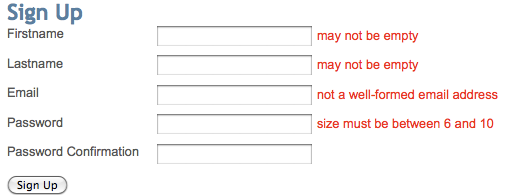
\includegraphics[width=9cm]{images/validation_registration}
        	\caption{Formular Validierung: Registration}
\end{figure}


Die Implementation der Methode validate basiert wie bereits gesagt auf dem Validation Framework und sieht folgendermassen aus:
\begin{lstlisting}[caption=Validation innerhalb der Klasse Persistence]
@Transient
private val validatorFactory = 
		Validation.buildDefaultValidatorFactory();

@Transient
private val validator = validatorFactory.getValidator();
  
def validate() = {
  validator.validate(this)
}
\end{lstlisting}

\subsection{Verwendung und Aufbau des Flex Clients}
F\"ur die Administration der Teams sowie auch f\"ur die Ferienplanung habe ich mich wegen von mir subjektiv empfundener besserer Usability und der M\"oglichkeit eines etwas besseren Software-Designs f\"ur Adobe Flex entschieden. 
\subsubsection{Architektur}
Die meisten User-Interfaces zeichnen sich, insbesondere durch die hohe Kopplung zwischen Komponenten, durch eine extrem schlechte Wartbarkeit aus. Diese Problematik kann in Applikationen verschiedenster Frontend-Technologien auftreten - egal ob Javascript, Flex, GWT oder Silverlight. Eine weitere Schwierigkeit bei diesen Applikationen sind die angemessene und zentrale Behandlung von auftretenden Events, die Verf\"ugbarkeit von Contexten und die Unterst\"utzung in der Anbindung an Backend-Systemen. Damit solche Problemstellungen f\"ur diesen Client minimiert werden k\"onnen, habe ich eine kurze Evaluation bestehender Flex-Frameworks durchgef\"uhrt und dabei die folgenden angeschaut:
\begin{itemize}
\item \textbf{Cairngorm\cite{Cairngorm} - } unter Flex 2 und 3 war Cairngorm noch ein Frameworks mit Fokus auf die MVC-Architektur von Client-Applikationen. Mittlerweile handelt es sich allerdings um ein breiteres Set von Guidelines, Tools und Bibliotheken. Welche sich frameworkunabh\"angig einsetzen lassen. Mittlerweile basieren viele dieser Bibliotheken auf anderen Dependency Injection und MVC Frameworks wie Parsley, Swiz, oder Spring ActionScript
\item \textbf{Mate\cite{Mate} - } in erster Linie wurde Mate f\"ur das Event-Handling entwickelt. Die Art und Weise der Konfiguration findet deklarativ via ein MXML statt und ist relativ unflexibel:

\begin{lstlisting}[caption=Event-Deklaration mit dem Mate Framework]
<EventHandlers type="{MessageEvent.GET}">
  <RemoteObjectInvoker 
    instance="{services.helloService}" 
    method="sayHello" 
    arguments="{event.name}">
    <resultHandlers>
      <CallBack 
        method="handleResult" 
        arguments="{resultObject.text}"/>
    </resultHandlers>
    <faultHandlers>
      <CallBack 
        method="handleFault" 
        arguments="{fault.faultDetail}"/>
    </faultHandlers>
    </RemoteObjectInvoker>
</EventHandlers>
\end{lstlisting}

\item \textbf{Switz\cite{Swiz} - }ist meines Erachtens das flexibelste und am elegantesten zu konfigurierende Framework. Es stellt folgende drei Hauptfunktionalit\"aten zur Verf\"ugung:
\begin{itemize}
	\item \textbf{Dependency Injection} als Basis zur Inversion of Control anhand eines Beispieles. Beans und somit der applikationsweite Context werden in einer MXML-Datei definiert:
\begin{lstlisting}[caption=Swiz: Bean Deklaration]
<swiz:BeanProvider ...>
  <fx:Declarations>
    <core:Context id="context"/>
  </fx:Declarations>
</swiz:BeanProvider>
\end{lstlisting}

Objekte k\"onnen nun in beliebeigen MXML-Dateien oder ActionScript Klassen injected werden - selbst two-way Bindings sind m\"oglich:
\begin{lstlisting}[caption=Swiz: Bean Injection]
[Inject(source="context.selectedTeam", 
        bind="true",
        twoWay="true")]
public var selectedTeam:Team = null;
\end{lstlisting}
\item \textbf{Event Handling} zur entkopplung von Mediator und Observer. Events werden mit der Methode dispatchEvent(Event e) des Interfaces IEventDispatcher geworfen werden. MXML sind grunds\"atzlich von diesem Typ, in normalen ActionScript-Klassen kann ein entsprechender Dispatcher injected werden. Um sich f\"ur Events zu registrieren ist eine Methode mit folgender Signatur und Annotation zu implementieren:

\begin{lstlisting}[caption=Swiz: Event Observer]
[Mediate( event="Events.SEARCH_USERS", 
          properties="term" )]
public function searchUsers( term:String) : void
{
//...
}
\end{lstlisting}
Hier wird das Property term des geworfenen Events zus\"atzlich der Methode als Argument \"ubergeben.
\item Einfacher Lifecycle f\"ur asynchrone Aufrufe auf Remote Systeme.
\end{itemize}
\end{itemize}

Aufgrund der Einfachheit des Swiz-Frameworks, der Flexibilit\"at und der eleganten Konfiguration habe ich mich gegen Cairngorm und Mate entschieden und das Event-Handling sowie Context und Dependency Injection mit Swiz implementiert.

\subsubsection{Kommunikation mit dem Backend}
Flex-Applikationen werden als Flash-Dateien dem Browser gesendet und laufen innerhalb der Flash Runtime Umgebung. Verglichen mit HTML 4.0.1 und XHTML 1.0 hat man mit Flex die M\"oglichkeit, Daten respektive Zust\"ande clientseitig zu Speichern.
In meinem Fall wird der Flex-Client innerhalb der Lift-Applikation eingebettet und kommuniziert mit dem Backend via \textbf{RESTful Webservices}. REST ist ein Architekturstil f\"ur Hypermedien wie das World Wide Web und legt nahe, jede Ressource mit einer eigenen URI anzusprechen. Operationen auf Ressourcen werden mittels HTTP Methoden  wie PUT, DELETE, POST,GET, HEAD, etc. zu verwenden.\cite{wiki:rest} Innerhalb der Browser-Umgebung ist die Verwendung von POST und GET m\"oglich, die anderen Methoden stehen allerdings nicht in allen Browsern zur Verf\"ugung. Zu diesem Zweck werden bei meinem Prototypen PUT- und DELETE-Requests mit dem HTTP-Header  ''X-HTTP-Method-Override'' ausgestattet und als eigentliche POST-Requests gesendet. Die Applikation merkt serverseitig von diesem Header nichts, da er bereits in der Filter-Kette zuvor die richtige Methode auf dem Request setzt. F\"ur weitere Informationen siehe:
\begin{itemize}
\item ch.plannr.common.http.WrappedRequest.java (server)
\item Klasse ch.plannr.common.http.RequestWrapperFilter.scala (server)
\item web.xml (server)
\item ch.plannr.service.HttpServiceFactory (client)
\end{itemize}
REST definiert grunds\"atzlich nicht, in welcher Form daten \"ubertragen werden m\"ussen.  M\"ogliche Formate w\"aren JSON und XML. Es war naheliegend, aufgrund der XML-Unterst\"utzung in Scala, dieses Format zu nehmen. F\"ur eine weitere Applikation w\"urde ich den Einsatz von BlazeDS\cite{blazeDs}\cite{IntegratingBlazeDsLiftweb} oder GranitDS\cite{graniteDs} p\"ufen.

Zu Beginn habe ich die \textbf{Authentifizierung} der Webservice-Aufrufe \"uber Basic Authentication gemacht. Dies h\"atte in der Praxis den wesentlichen Nachteil, dass prinzipiell alle Aufrufe verschl\"usselt werden m\"ussen\footnote{Bei Basic Authentication wird Benutzernamen und Passwort in der Form ``username:password'' im Base-64 Format \"ubermittelt}.
Nun habe ich die Authentifizierung auf eine Form-Authentication umgestellt, bei der die Benutzer-Identifikation respektive in meinem Fall die Email-Adresse in der Session gespeichert wird. Somit muss nur der Login-Formular Submit via das Https-Protokoll laufen.

\subsection{Navigation}
Da die Ferienplanung und Administration der Benutzer vollumf\"anglich in Flex implementiert ist, basiert auch die Navigation dieser Beiden Use Cases auf Flex Komponenten wie Tab-Panels sowie States und Transitions (siehe: ``\ref{implementation:ferienplanung} \titleref{implementation:ferienplanung}'').  Ausserhalb ist die Navigation mittels der Lift-Sitemap implementiert. Wie bereits unter ``\ref{lift:sitemap} \titleref{lift:sitemap}'' angek\"undigt bezieht sich die Lift-Sitemap nicht nur auf das Verlinken von Seiten, sondern auch f\"ur die Zugriffskontrolle. Die Struktur des Menus sieht folgendermassen aus:

\begin{spacing}{0.5}
  \begin{longtable}{|p{2cm}|p{5cm}|p{6cm}|}
      \caption{Navigation und Menustruktur}\\
\hline
  \textbf{Name} & \textbf{Link} & \textbf{Constraints}\\
  \hline
  Home & /index & keine\\
  \hline
  Manager & /manager & Benutzer angemeldet\\
  \hline
  Login & /user\_mgt/login & Benutzer nicht angemeldet\\
  \hline
  Benutzer registrieren & /user\_mgt/sign\_up & Benutzer nicht angemeldet\\
  \hline
  Passwort verloren & /user\_mgt/lost\_password & Benutzer nicht angemeldet\\
  \hline
  Logout & /user\_mgt/logout & Benutzer angemeldet\\
  \hline
 Passworter reset & /user\_mgt/reset\_password & Benutzer angemeldet\\
  \hline
  Benutzer editieren & /user\_mgt/edit & Benutzer angemeldet\\
  \hline
  Passwort \"andern & /user\_mgt/change\_password & Benutzer angemeldet\\
  \hline
  \end{longtable}
\end{spacing}

Das Menu wird aus einer Liste von Menu-Eintr\"agen in der Klasse Boot.scala definiert und in die SiteMap gesetzt. Die Zugriffssteuerung wird \"uber die LocParams implementiert die sich in den Menu Instanzen befinden. 
 
 \section{Details zur Implementation der Use Cases}
 \subsection{Benutzermanagement}
Sofern man bei der Entwicklung von Webapplikationen mittels Lift den Persistenz-Provider Mapper ausw\"ahlt, erh\"alt man Benutzerverwaltung inklusive Login-, Registrierung- und Passwort-Reset-Mechanismus mitgeliefert und kann diesen relativ flexibel erweitern. Da ich mich allerdings aus den oben beschriebenen Gr\"unden f\"ur JPA und gegen Mapper entschieden habe, musste ich diese Funktionalit\"at selber implementieren. Dies habe ich auf der Basis des ProtoUsers, MegaProtoUsers und MetaMegaProtoUser vom Mapper-Framework getan. Zur Beschreibung wie die Benutzerdaten zwischen Formularen und dem Backend ausgetauscht werden, eine kurze Erl\"auterung wie die Funktionalit\"at Passwort-Reset funktioniert:

\begin{lstlisting}[caption=Implementation Funktionalit\"at Passwort-Reset]
def passwordReset(id: String) =
    findById(id.toLong) match {
      case Full(user) =>
        def finishSet() {
          val violations = user.validate
          if (violations.size == 0)
            user.merge
          else {
            val node: NodeSeq = violations
            S.error(node)
            S.redirectTo("/")
          }
        }

        bind("user", HtmlTemplate.passwordResetXhtml,
          "pwd" -> 
            password_*("", (p: List[String]) =>
              user.password = p.head),
          "submit" -> 
            submit(S.??("set.password"), finishSet _))
      case _ => 
        S.error(S.??("password.link.invalid")); 
        S.redirectTo(homePage)
    }
\end{lstlisting}
Die Methode zum Reset des Passworts wird vom Menu respektive der Lift-Internen SiteMap Funktionalit\"at (siehe unter: ``\ref{lift:sitemap} \titleref{lift:sitemap}'') aufgerufen. M\"oglich ist dies nur, wenn der Benutzer angemeldet ist..  Der R\"uckgabewert der passwordReset-Methode ist ein Objekt vom Typ scala.xml.NodeSeq, welches das eigentliche Formular repr\"asentiert. Eingabefelder werden nicht in reinem HTML definiert, sondern via die Verwendung der Methoden text, password, usw. Diese Methoden der Klasse SHtml registrieren zum einen eine Callback-Funktion, zum anderen geben sie das auszugebenden Xml-Element als scala.xml.Elem zur\"uck. Beim \"Ubermitteln des Formulars wird dann die entsprechend zu einer definierten ID registrierte Callback-Funktion mit dem vom Benutzer eingegebenen Wert aufgerufen. Zum einen wird somit f\"ur die Textfelder der Wert hinterlegt, zum anderen via die Methode finishSet der Benutzer validiert und gespeichert. 

Alle Formulare der Benutzerverwaltung sind in etwa auf diese Weise implementiert. 


 
\subsection{Ferienplanung und Teammanagement}\label{implementation:ferienplanung}
Die Prozesse der Teamadministration und Ferienplanung sind unter ``\ref{prozess:ferien} \titleref{prozess:ferien}'' und  ``\ref{prozess:team} \titleref{prozess:team}'' beschrieben. Aufgrund der folgenden drei Gr\"unde habe ich mich entschieden, beide Teile in Flex zu implementieren:
\begin{itemize}
\item \textbf{Usability: } Usability bezeichnet die vom Nutzer erlebte Nutzungsqualit\"at (respektive User Experience) bei der Interaktion mit einem System\cite{wiki:usability}. Heutzutage erreicht man dies mit der Verwendung von Technologien wie Ajax, Flex, Silverlight, oder andere. Der Benutzer erf\"ahrt die Webseite wie als eine auf seinem Rechner installierte Applikation:
\begin{itemize}
\item kurze Ladezeiten
\item Interaktion mit dem Server findet statt indem nur Teile der Seite ausgetauscht werden.
\end{itemize}
\item \textbf{Aufwand: }Der Aufwand um Administrationsoberfl\"achen zu implementieren ist vergleichsweise geringer. Man muss allerdings auch ber\"ucksichtigen, dass die Kommunikation mit dem Backend respektive das Testen der Schnittstelle zum Backend trotzdem eine Menge Zeit in Anspruch nimmt.
\item \textbf{Kalender: } Die Verwendung des Flex Kalenders ``IBM Eloxier'' erschien mir als angemessen (Siehe Abschnitt ``\ref{evaluation:kalender} \titleref{evaluation:kalender}'')
\end{itemize}

\subsubsection{Evaluation Kalender}\label{evaluation:kalender}
Unter dem Namen ``Elixier'' verkauft IBM Flex Komponenten. Da ich bereits im Besitz der Standard-Lizenz war, habe ich mich f\"ur diesen Kalender entschieden. Die Enterprise Version beinhaltet zus\"atzlich noch ein Gantt-Chart \cite{wiki:gantt}, der f\"ur private doch relativ hohe Preis (dieser liegt momentan bei 3130 USD) hat mich allerdings von der Verwendung dieser Komponente gehindert.  Andere Widgets habe ich aufgrund meiner Meinung nach mangelnder Qualit\"at, Stabilit\"at oder Funktionalit\"at nicht verwendet:

\begin{itemize}
\item Simile Timeline\cite{simileTimeline}
\item Flex Calendar Components \cite{flexCalendar}
\end{itemize}


\subsection{Email-Versand (Notifikationen)}
\subsubsection{Use Cases}
Zu unterschiedlichen Zwecken m\"ussen  Emails an die Benutzer versendet werden. Die Email-Adressen gelten systemweit als Benutzer Identifikatoren und sind deshalb sowieso bereits beim Benutzer gespeichert. Nachfolgend eine Liste der Use Cases mit Email und der Stand der Implementation im Prototypen:
 \begin{longtable}{|p{3cm}|p{7cm}|p{3cm}|}
      \caption{Use Cases Email Versand}\\
\hline
  \textbf{Aktion} & \textbf{Beschreibung} & \textbf{Status der Implementation}\\
  \hline
  Signup&Nach der Registrierung wird zur Email-Validierung ein Email inklusive einem Link an den Benutzer versendet, \"uber welchen er den Account aktivieren kann. Im Link enthalten ist eine Zufallszahl so dass kein Missbrauch betrieben werden kann. & Nicht implementiert\\
  \hline
  Passwort vergessen&Sofern das Passwort vergessen geht, wird ein Email an den Benutzer versendet. \"Uber dieses Email kann das Passwort neu gesetzt werden. & Implementiert\\
  \hline
  Erfassung von Ferien durch den Mitarbeiter & Nachdem der Benutzer seine Ferienw\"unsche erfasst hat, geht ein Email an den Vorgesetzten, damit dieser die Eintr\"age \"uberpr\"ufen kann & Nicht implementiert \\
  \hline
  Status\"anderung durch Vorgesetzten & Nachdem der Vorgesetzte die Ferien \"uberpr\"uft und bewilligt, abgelehnt hat, wird der Mitarbeiter informiert & Nicht implementiert\\
  \hline
\end{longtable}
 
 \subsubsection{Technische Umsetzung}
 In meinem Fall l\"asst sich der Lift-Mail-Support, der sich innerhalb der Klasse net.liftweb.util.Mailer befindet, nicht nur \"uber die definition der Properties (mail.smtp.host, mail.username, mail.password) konfigurieren - ich muss zus\"atzlich den Authenticator (Mailer.authenticator) des Objekts Mailer setzen.

 Mails k\"onnen nun mit dem Aufruf der folgenden Methode versendet werden:
\begin{lstlisting}[caption=]
    Mailer.sendMail(From(emailFrom), 
                    Subject(signupMailSubject),
                    (To(user.email) :: 
                    xmlToMailBodyType(msgXml) ::
                    (bccEmail.toList.map(BCC(_)))): _*)
\end{lstlisting} 

Das erste Argument ist die Absender-Adresse, das zweite das Subject und das dritte eine Liste bestehend aus Empf\"anger, Carbon Copy (CC), Blind Carbon Copy (BCC) und Mailbodies (HTML, Plain Text). Die Liste wird vom Lift Framework beim Verwenden wieder in ihre Bestandteile aufgel\"ost und mit Empf\"anger und Subject versendet. 

\chapter{Entwicklung, Build und Deployment}

\section{Build-System}Maven als Build-System basiert ebenfalls auf einem Plugin-Konzept und unterst\"utzt in den verschiedensten Bereichen des Build-Managements. Nicht zuletzt dank dem Grundsatz ``Convention over Configuration'' l\"asst es sich auf allen Plattformen im Nu deployen. Maven \"ubernimmt bei diesem Projekt eine vielzahl an Funktionen:

\begin{itemize}
\item \textbf{Dependency Management: } Maven l\"adt die im pom.xml definierten Abh\"angigkeiten von \"offentlichen Repositories. 
\item \textbf{Support Entwicklungsumgebung:  } Die grosse Verbreitung von Maven hat dazu gef\"uhrt, dass Entwicklungsumgebungen Adapter oder Plugins daf\"ur entwickelt haben vomit sich solche Projekte automatisch innerhalb der IDE konfigurieren. Dazu geh\"ort das Hinzuf\"ugen von Abh\"angigkeiten in den Source- und Build-Pfad, das korrekte setzen von Ausgabe-Ordner. 
\item \textbf{Clean, Compile, Package: }Der gesamte Build-Prozess f\"urs Test-System findet mit Maven statt. Bei der Entwicklung werden die Klassen allerdings von der Entwicklungsumgebung kompilliert - diese beschriebenen Targets sind deshalb da nicht n\"otig. 
\item \textbf{Profil Management - } Maven ist von Grund auf f\"ahig, verschiedene Profile zu definieren. Profile kann man beispielsweise dann verwenden, wenn Applikationen f\"ur Entwicklung, Test, Produktion in unterschiedlichen Umgebungen laufen. Dann gilt es meistens, unterschiedliche Konfigurationen zu verwenden. Profile brauche ich um folgende Probleme zu l\"osen:\begin{itemize}
\item Der Datenbank-Zugriff wird in der Entwicklungsumgebung direkt \"uber JDBC gemacht, in der Testumgebung auf der Stax-Cloud wird eine von Servern verf\"ugbare Datasource verwendet.
\end{itemize}
\end{itemize}
\section{Entwicklungsumgebung}
W\"ahrend der Entwicklung hilft Maven vorallem im Bereich des Dependency Managements - Abh\"angigkeiten werden automatisch geladen, das Projekt kann nach der \"Offnung sofort kompiliert und gestartet werden. Die meisten Funktionalit\"aten im Backend habe ich Test-Driven mit Scala-Specs entwickelt, ohne dass ich die Funktionalit\"at jedesmal im Browser nachvollzog. Tests kann man auf verschiedene Arten ausf\"uhren:
\begin{itemize}
\item Maven per Default unterst\"utzt die Ausf\"uhrung von JUnit-Tests, mit Plugins k\"onnen allerdings auch Scala-Specs oder andere Tests ausf\"uhren.
\item Entwicklungsumgebungen welche Scala unterst\"utzen, bringen meistens auch Funktionalit\"at zum Testen (Ausf\"uhrung von Scala Specs oder Scala Unit  Tests). 
\item Die Scala-Gemeinde richtet sich mehr und mehr auf das Simple Build Tool\cite{SimpleBuildTool} aus. Es handelt sich dabei um ein Tool welches ebenfalls Dependency Management, Test, Build, usw. unterst\"utzt und sich gegebenenfalls auch mit Maven kombinieren l\"asst. Bei der Entwicklung hat das Tool mir geholfen, die Tests auszuf\"uhren, indem es kontinuierlich auf \"Anderungen wartet, neu Kompiliert und entsprechend die Tests neu ausf\"uhrt. Das somit schnelle Feedback kann den Entwicklungsprozess massiv beschleunigen.\end{itemize}


\section{Test- und Produktiv-Umgebung}
Um die Applikation auch der Breiten Masse verf\"ugbar zu machen, habe ich sie auf der Cloud-Plattform namens Stax\cite{Stax} deployt. Bei der Verfolgung von Twitter-Nachrichten verschiedener Personen und Diensten bin ich auf diese Plattform aufmerksam geworden und die Einfachheit des Deployments hat mich sehr \"uberrascht.

F\"ur das Deployment auf diese Plattform musste ich folgende \"Anderungen durchf\"uhren:
\begin{itemize}
\item \textbf{Stax-Konfiguration f\"ur Maven - } F\"ur Maven ist ein Stax-Plugin vorhanden, das mittels der folgenden Zeilen im pom.xml konfiguriert werden muss: 

\begin{lstlisting}[caption=Konfiguration Maven mit Stax]
<build>
  <plugins>
    <plugin>
      <groupId>net.stax</groupId>
      <artifactId>stax-maven-plugin</artifactId>
    </plugin>
  ...
  </plugins>
</build>
\end{lstlisting}
Schlussendlich ist es m\"oglich, die Applikation mittels dem folgenden Kommando zu deployen:
\begin{lstlisting}[caption=Befehl Deployment Stax]
mvn clean stax:deploy -Pprod -Dstax.appid=plannr
\end{lstlisting}
\item \textbf{Stax-Konfiguration des Web Archives - } Wars f\"ur die Stax Plattform m\"ussen ein zus\"atzliches Xml mit dem namen stax-web.xml beinhalten. 
\item \textbf{Datasource Anbindung - } Via das Web-Interface von Stax kann eine neue MySql Datenbank auf der Cloud angelegt werden. Um der Applikation den Zugriff auf diese Datenbank zu erm\"oglichen, wird diese einerseits im stax-web.xml als auch im web.xml definiert. Die Aufl\"osung der Datasource wird zur Laufzeit \"uber den JNDI-Namen gemacht, der im persistence.xml definiert ist.
\item \textbf{Konfiguration JPA -} Damit sich der Persistenz-Provider nicht wie w\"ahrend der Entwicklungszeit direkt \"uber JDBC mit Url, Benutzernamen und Passwort verbindet, wird im Profilabh\"angigen persistence.xml f\"ur Test- und Produktiv-Umgebung die im web.xml als Ressource definierte Datasource verwendet. 
\end{itemize} 

Der Pfad f\"ur diese Dateien werden nur mit der Aktivierung \"uber das Maven-Profil geladen und \"uberschreiben die bereits bestehenden.







	

\part{R\"uckblick}
\chapter{Auswertung und Fazit der verwendeten Technologien}
\section{Scala}\label{auswertung:scala}
Subjektiv gesehen hat man stark das Gef\"uhl, dass Funktionale Sprachen, insbesondere Sprachen auf der Java- oder Dot-Net-Plattform in letzter Zeit das Interesse der Entwicklergemeinde auf sich gezogen haben. Auch der Tiobe Index \cite{tiobe} hat diese Tendenz in den letzten Monaten best\"atigt. In wenigen Worten haben die erw\"ahnten Sprachen oft eine ``smartere'' Syntax (siehe Abschnitt ``\ref{imperativ-deklarativ} \titleref{imperativ-deklarativ}''), lassen sich im Grossen und Ganzen besser parallelisieren und k\"onnen in vielen Bereichen von bestehenden Bibliotheken und Frameworks ihrer bereits etablierten Plattformen profitieren. Man kann wohl sagen, dass sich die \"aquivalenten Problemstellungen, bis anhin implementiert in Sprachen wie Java, in Zukunft auch mit Scala umgesetzt werden k\"onnen. Trotzdem kann die Effizienz w\"ahrend der Entwicklung sich, aufgrund des massiv schlechteren Tool Supports\footnote{}, noch nicht mit dem Entwicklungsprozessen, wie sie bei Java Applikationen der Fall sind, messen. In den folgenden Abschnitten m\"ochte ich mich auf die Syntax und Ausdrucksst\"arke beziehen:
\subsection{Typisierung}
Zu diesem Thema scheiden sich ja bekanntlich die Geister - und ich habe nicht den Anspruch, ein Fazit pro oder kontra typisierter Sprachen zu ziehen. Bef\"urworter dynamischer Sprachen anerkennen zwar die Typsicherheit zur Kompilierzeit, kalkulieren aber den daf\"ur zu bezahlenden Preis mit schlechtem Code Smell.  Die n\"achste Tabelle soll zeigen, dass die in diesem Zusammenhang erw\"ahnten Argumente nichts mit der Typisierung zu tun haben. 
  \begin{longtable}{|p{4cm}|p{4cm}|p{4cm}|}
      \caption{Genannte Gr\"unde gegen typisierte Sprachen}\\
\hline
  \textbf{Genannte Gr\"unde} & \textbf{Auswirkung in Java} & \textbf{Scala}\\
  \hline
  DRY-Prinzip\footnote{Don't Repeat Yourself, ein Grundsatz f\"ur guten Code Smell} \newline repetit. Informationen& 
  Explizite Typangabe: \newline String s = ''explizit'' & Implizite Typisierung \newline val s = ''implizit''\\
  \hline
  Verbosit\"at & z. Bsp. annonyme Innerklassen wie Comparator & Funktionsobjekte, Closures \\
  \hline
\end{longtable}

\subsection{Sprachdesign und Syntax}
Bei der Einarbeitung in Scala f\"allt einem sofort folgendes auf:
\begin{itemize}
\item Scala ist statisch, stark typisiert, hat hervorragende Type Inference
\item Scala wurde von vielen Sprachen beeinflusst: Java, ML, Haskell
\item Scala wurde von Personen entwickelt, die schon lange im Sprachdesign t\"atigt sind. Ich begr\"unde diese Aussage mit der wunderbaren Konsistenz 
\begin{itemize}
\item hinsichtlich Operator Overloading, respektive alles ist eine Methode.
\item hinsichtlich der Verwendung von Collections wie List und Map. 
\end{itemize}
\item Scala beinhaltet grossartige Konzepte wie
\begin{itemize}
\item Pattern Matching.
\item Implizit Conversions.
\end{itemize}
\end{itemize}

\subsection{Tool Support}
Nebst der Tatsache, dass Scala Code um L\"anger pr\"agnanter\footnote{t\"ont in Englisch besser: concise} ist als Java, wird man w\"ahrend der Entwicklung mit der Tatsache konfrontiert, dass das Tooling, die Programme die einen w\"ahrend der Entwicklung unterst\"utzen, noch lange nicht auf dem Level von Java ist: 
\begin{itemize}
\item der Scala Compiler ist aktuell noch nicht gen\"ugend schnell
\item die Code-Vervollst\"andigung erkennt nur ganz einfache Zusammenh\"ange
\end{itemize}

\subsection{Verbreitung}
Trotz der Sch\"onheit und Kosistenz dieser Sprache, bin ich sehr gespannt, wie sie sich in der nahen Zukunft auch in der Industrie festsetzen wird. Ich bin der Meinung, dass die Verbreitung von Scala ohne ein Framework im Bereich des Internets sehr schwierig sein wird. Web Frameworks k\"onnen sich nur dann verbreiten, wenn durch eine augekl\"ugelte Erweiterbarkeit ein \"Okosystem rundherum entsteht. So dass Websiten in kurzer Zeit und entsprechend kosteng\"unstig entstehen k\"onnen. Als Paradebeispiel in diesem Bereich sehe ich Rails aber auch Grails (siehe Abschnitt ``\ref{auswertung:groovy-lift} \titleref{auswertung:groovy-lift}''. 



\section{Lift Framework}\label{auswertung:lift}

\subsection{Vergleich von Lift mit Grails}\label{auswertung:groovy-lift}



\chapter{Analyse der Arbeit auf der Basis der Aufgabenstellung}
\section{Zielerreichung}
\subsection{Entwicklung und Deployment}

\section{Optionale Ziele}

\subsection{Performance Tests}

\subsection{Internationalisierung}

\subsection{Search Engine Optimization}

\subsection{Usability}



\begin{thebibliography}{widest entry}

\bibitem{BawiSwPm} Hindel, H\"ormann, M\"uller, Schmied, \emph{Basiswissen Software-Projektmanagement}

\end{thebibliography}
\lstlistoflistings
\listoffigures
\listoftables
\part{Anhang}
\appendix
\chapter{Glossar}
  \begin{longtable}{|p{4cm}|p{10cm}|}
      \caption{Glossar}\\
\hline
  Wort & Beschreibung\\
  \hline
  & \\
  \hline
  
  \end{longtable}



\chapter{Journal}


\section{Phase Implementation Backend}
\begin{spacing}{0.5}
  \begin{longtable}{|p{4cm}|p{10cm}|}
      \caption{Journal Implementation Backend}\\
\hline
  Datum & Eintrag\\
  \hline
  7. August 2010 & 
  \begin{itemize}
  \item Projekt Setup Client und Server 
  \item Initialer Commit ins Git Repository unter http://github.com/schmidic
  \end{itemize}\\
  \hline

  13. August 2010 & 
  \begin{itemize}
  \item Installation des Persistenz Providers (Hibernate und JPA)
  \end{itemize}\\
  \hline
  
  14. August 2010 & 
  \begin{itemize}
  \item Authentifizierung und Authorisierung via Basic Authentication
  \item Implementation REST Support in f\"ur Browser, abfrage des X-HTTP-Method-Override Headers, da Browser nicht wirklich PUT und DELETE requests unterst\"utzen.
  \end{itemize}\\
  \hline
  
  16. August 2010 & 
  \begin{itemize}
  \item Registrierung und Login Webservice
  \end{itemize}\\
  \hline

  17. August 2010 & 
  \begin{itemize}
  \item Erarbeiten des Entity Relationship Models
  \item Mapping der Domain-Klassen auf das ERM via JPA
  \end{itemize}\\
  \hline
  
  18. August 2010 & 
  \begin{itemize}
  \item Webservices zur Administration der Teams und User
  \item Laden von Fixtures mittels import.sql
  \end{itemize}\\
  \hline
  
    20. August 2010 & 
  \begin{itemize}
  \item Erweiterung der bestehenden Webservices
  \end{itemize}\\
  \hline
  
   22. August 2010 & 	
  \begin{itemize}
  \item Webservice zur Administration der Ferien
  \item Anpassung des Persistenz Mappings
  \end{itemize}\\
  \hline
   27. August 2010 & 
  \begin{itemize}
  \item Konfiguration von Maven-Profilen f\"ur das Deployment auf STAX\footnote{http://stax.net}
  \end{itemize}\\
  \hline
    \end{longtable}
\end{spacing}
  
  \section{Phase Implementation Frontend}
  \begin{spacing}{0.5}
  \begin{longtable}{|p{4cm}|p{10cm}|}
      \caption{Journal Implementation Frontend}\\
\hline
  Datum & Eintrag\\
  \hline
  24. August 2010 & 
  \begin{itemize}
  \item Evaluation unterschiedlicher Actionscript Frameworks (Mate\footnote{http://mate.asfusion.com}, Swiz \footnote{http://swizframework.org}, Cairngorm\footnote{http://opensource.adobe.com/wiki/display/cairngorm/Cairngorm}) f\"ur Dependency Injection und Event Handling. Entscheidung zugunsten Swiz augrund der folgenden Eigenschaften: Flexibilit\"at, Leistungsf\"ahigkeit (Context, TwoWay-Bindings, Injection, Event-Dispatching), Annotation-Support, Service Integration.
  \item Initialer Commit ins Git Repository unter http://github.com/schmidic
  \end{itemize}\\
  \hline
  
 26. August 2010 & 
  \begin{itemize}
  \item Browser sendet 401 bei Nicht-Authorisierung - dies f\"uhrt zu einem Browser-Popup f\"ur Benutzername und Passwort. Noch keine L\"osung gefunden. 
  \end{itemize}\\
  \hline
  
 27. August 2010 & 
  \begin{itemize}
  \item Fertigstellung der Administrations-Ansicht
  \item Integration des Schedulers von ILOG Elixier
  \end{itemize}\\
  \hline
    \end{longtable}
  \end{spacing}
  
  
    \section{Phase Dokumentation}
  \begin{longtable}{|p{4cm}|p{10cm}|}
      \caption{Journal Dokumentation}\\
\hline
  Datum & Eintrag\\
   \hline
  19. September 2010 & Grundlagen\\\hline
    19. September 2010 & Entity Relationship Model\\\hline
    20. September 2010 & Grundlagen\\\hline
    21. September 2010 & Grundlagen\\\hline
    \end{longtable}
  


\end{document}
